\documentclass[../sparc.tex]{subfiles}
\graphicspath{{\subfix{../images/}}}
\begin{document}

%%%%%%%%%%%%%%%%%%%%%%%%%%%%%%%%%%%%%%%%%%%%%%%%%%%%%%%%%%%%%%%%%%%%%%%%%%%%%%%%
\section{Последовательный порт}
\index{Электроника!Последовательный порт}
\label{section:serial-port}

Последовательный порт в Arduino -- это тот самый USB-B, который мы подключаем
всякий раз, когда желаем включить наш микроконтроллер или загрузить в Arduino
какую-либо программу.  С помощью последовательного порта можно передавать данные
с Arduino на компьютер и наоборот.

\subsection{Основы работы с Arduino через последовательный порт}

Прежде, чем начать работать с последовательным портом, нам необходимо его
настроить; делается это следующим образом: в теле функции setup мы должны
написать:

\begin{minted}{cpp}
void setup() {
  Serial.begin(9600);
}
\end{minted}

В этом случае мы обеспечиваем обмен данными между компьютером и Arduino с
указанной скоростью, где 9600 -- это скорость, с которой мы передаем данные на
персональный компьютер в \emph{бодах} (битах в секунду.) Обычно данный параметр
принимает одно из следующих значений: 300, 600, 1200, 2400, 4800, 9600, 14400,
19200, 28800, 38400, 57600, 115200.

\subsection{Передача данных на компьютер}

Теперь попробуем передать какие-нибудь данные на компьютер. В качестве примера
мы просто отправим строку ``Hello, world!'' по последовательному порту. Для
начала пропишем настройку порта в функции \texttt{setup}:

\begin{minted}{cpp}
void setup() {
  Serial.begin(9600); // устанавливаем скорость порта
}
\end{minted}

А вот так в нашем случае выглядит функция \texttt{loop}:

\begin{minted}{cpp}
void loop() {
  Serial.println("Hello World");
  delay(1000); // ждём 1000 мс перед следующей отправкой
}
\end{minted}

Результат выполнения программы можно увидеть, открыв монитор порта в Arduino IDE
-- это можно сделать из меню ``Инструменты'' (``Tools''), выбрав пункт ``Монитор
порта''.

Кроме того, открыть монитор порта можно, нажав комбинацию клавиш \hotkey{Ctrl +
  Shift + M}.

Внешний вид монитора порта показан на рис. \ref{fig:arduino-ide-serial-monitor}.
В заголовке окна указано название устройства, которым представлена плата Arduino
в системе и через которое компьютер взаимодействует с платой.

Ниже следует строка ввода данных для передачи их на Arduino.

Основную часть экрана занимает область отображения данных, приходящих с Arduino
на компьютер.

В нижней части окна находится панель настроек.

Цифрами на рисунке указаны:
\begin{enumerate}
\item Строка ввода данных для передачи их с компьютера на Arduino.
\item Кнопка ``Отправить'' (англ. ``Send''), по нажатию на которую данные,
  введённые в строку слева, будут отправлены на Arduino.
\item Отметка о времени прихода данных с Arduino на компьютер.
\item Принятые с Arduino данные.
\item Опция ``Автопрокрутка'' (англ. ``Autoscroll'').  Если данная опция
  включена, то основная область окна, отображающая приходящие данные,
  автоматически прокручивается таким образом, чтобы самые последние данные были
  всегда вверху.
\item Опция ``Показать отметку о времени'' (англ. ``Show timestamp'') позволяет
  включить отображение отметок о времени (цифра \textbf{3} на рисунке).
\item Настрока перевода строк, используемых при коммуникации с Arduino.  Здесь
  можно выбрать один из вариантов: ``No line ending'' (Без перевода строк),
  ``Newline'' (Перевод строки), ``Carriage return'' (Символ ``возврат каретки'')
  и ``Both NL \& CR'' (режим, в котором в роли конца строки используются сразу
  два символа -- перевод строки и возврат каретки.)  Данная опция влияет на то,
  какую последовательность символов монитор порта считает за конец строки
  данных.
\item Настройка скорость передачи данных в бодах (битах в секунду).
  По-умолчанию выставлена в 9600 бод.  Если значение данной настройки не
  соответствует тому, который был указан в программе, работающей на Arduino
  (через \texttt{Serial.begin}), то тогда на в мониторе порта вместо данных
  будут отображаться ``кракозяблики'' (иными словами, какая-то нечитаемая
  последовательность символов.)
\item Кнопка ``Очистить вывод'' (англ. ``Clear output'') позволяет очистить окно
  монитора порта.
\end{enumerate}


\begin{figure}[ht]
  \centering
  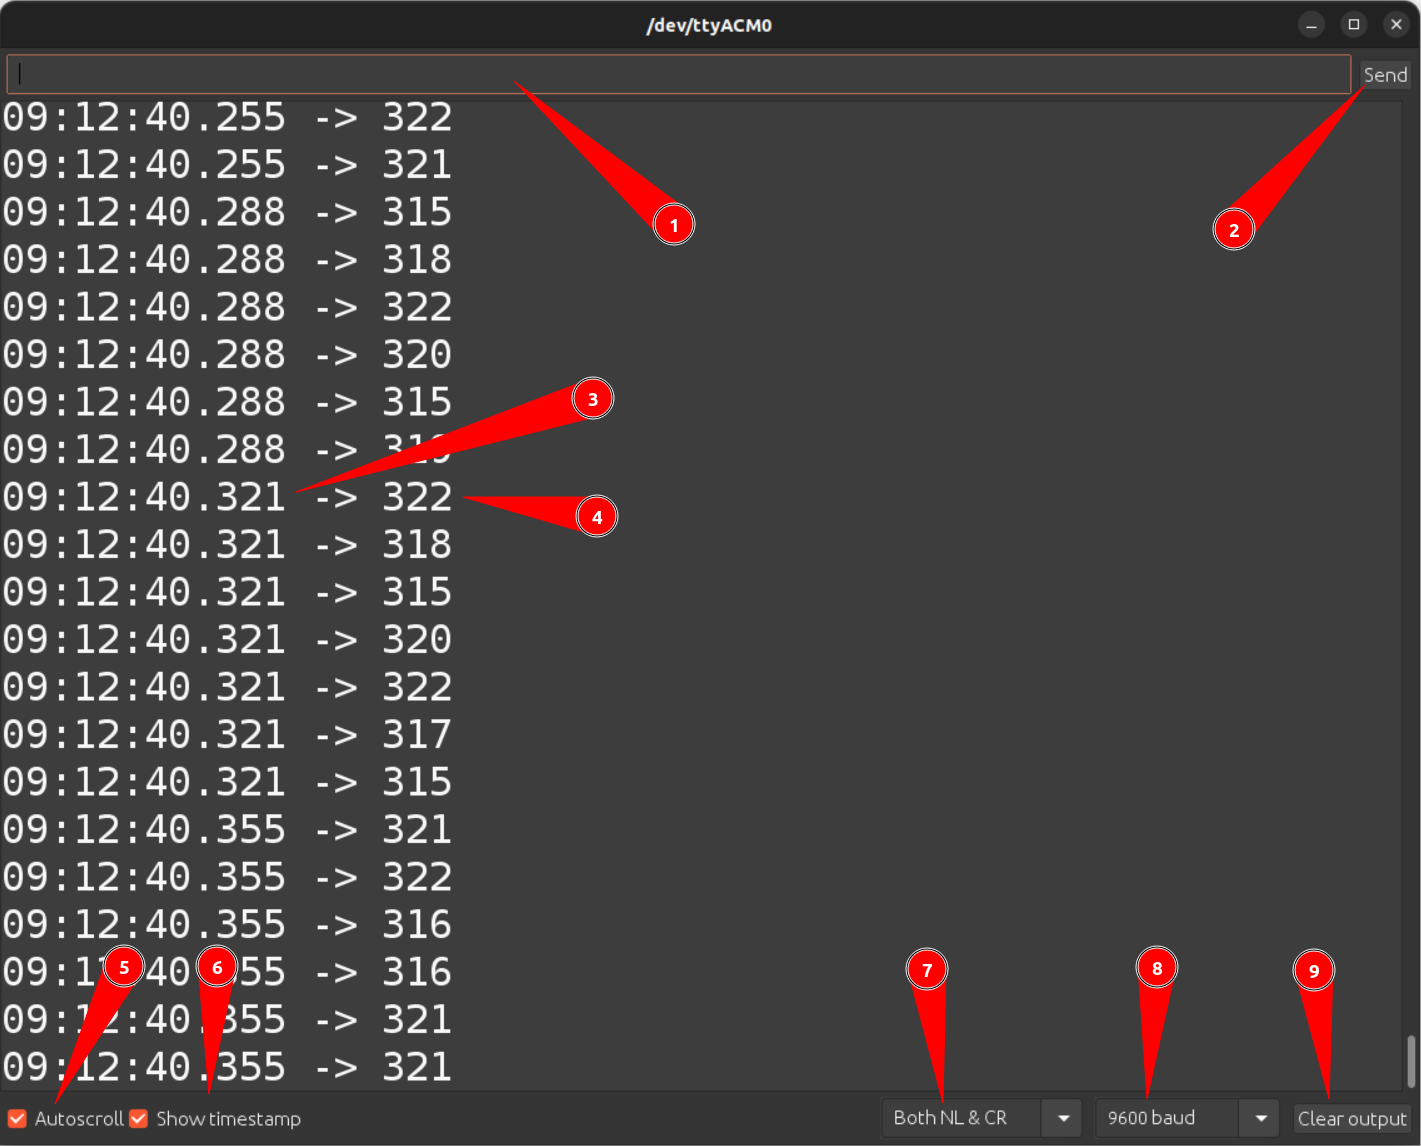
\includegraphics[width=10cm]{arduino-ide-serial-monitor}
  \caption{Монитор порта (``Serial Monitor'') в Arduino IDE 1.8.19.}
  \label{fig:arduino-ide-serial-monitor}
\end{figure}

Передачу данных с Arduino на компьютер можно использовать в множестве разных
задач. Примером одной из таких задач является простейший способ отладки программ
-- с помощью вывода информации о работе программы в Arduino на последовательный
порт. Иными словами, вместо того, чтобы пытаться самим понять, что же пошло не
так и почему что-то не работает, мы просим Arduino саму рассказывать нам, что
она делает.

\subsection{Визуализация данных}

При большом объёме данных неудобно смотреть их в ``Мониторе порта'' -- от
большого количества чисел может буквально ``рябить в глазах''.  В подобных
случаях нам поможет визуализация данных.

Визуализация данных является очень важной составляющей их анализа -- графическое
представление безликих чисел даёт возможность быстро и ёмко охватить их ``одним
взглядом'', и часто именно это помогает выявить закономерности в данных, в ином
случае скрытых от глаз человека.

Есть разные способы визуализировать данные; одним из таких способов, доступных
нам, является ``Плоттер по последовательному соединению'', который позволяет
прямо из Arduino IDE получить вывод потока данных в виде графика.  Доступ к
``Плоттеру'' осуществляется через меню ``Инструменты'', в котором нужно выбрать
пункт ``Плоттер по последовательному соединению'', либо через комбинацию клавиш
\hotkey{Ctrl + Shift + L}.

Внешний вид плоттера по последовательному соединению показан на
рис. \ref{fig:arduino-ide-serial-plotter}.

Как и для монитора порта, в заголовке окна плоттера указано название устройства,
которым представлена плата Arduino в системе и через которое компьютер
взаимодействует с платой.

\begin{figure}[ht]
  \centering
  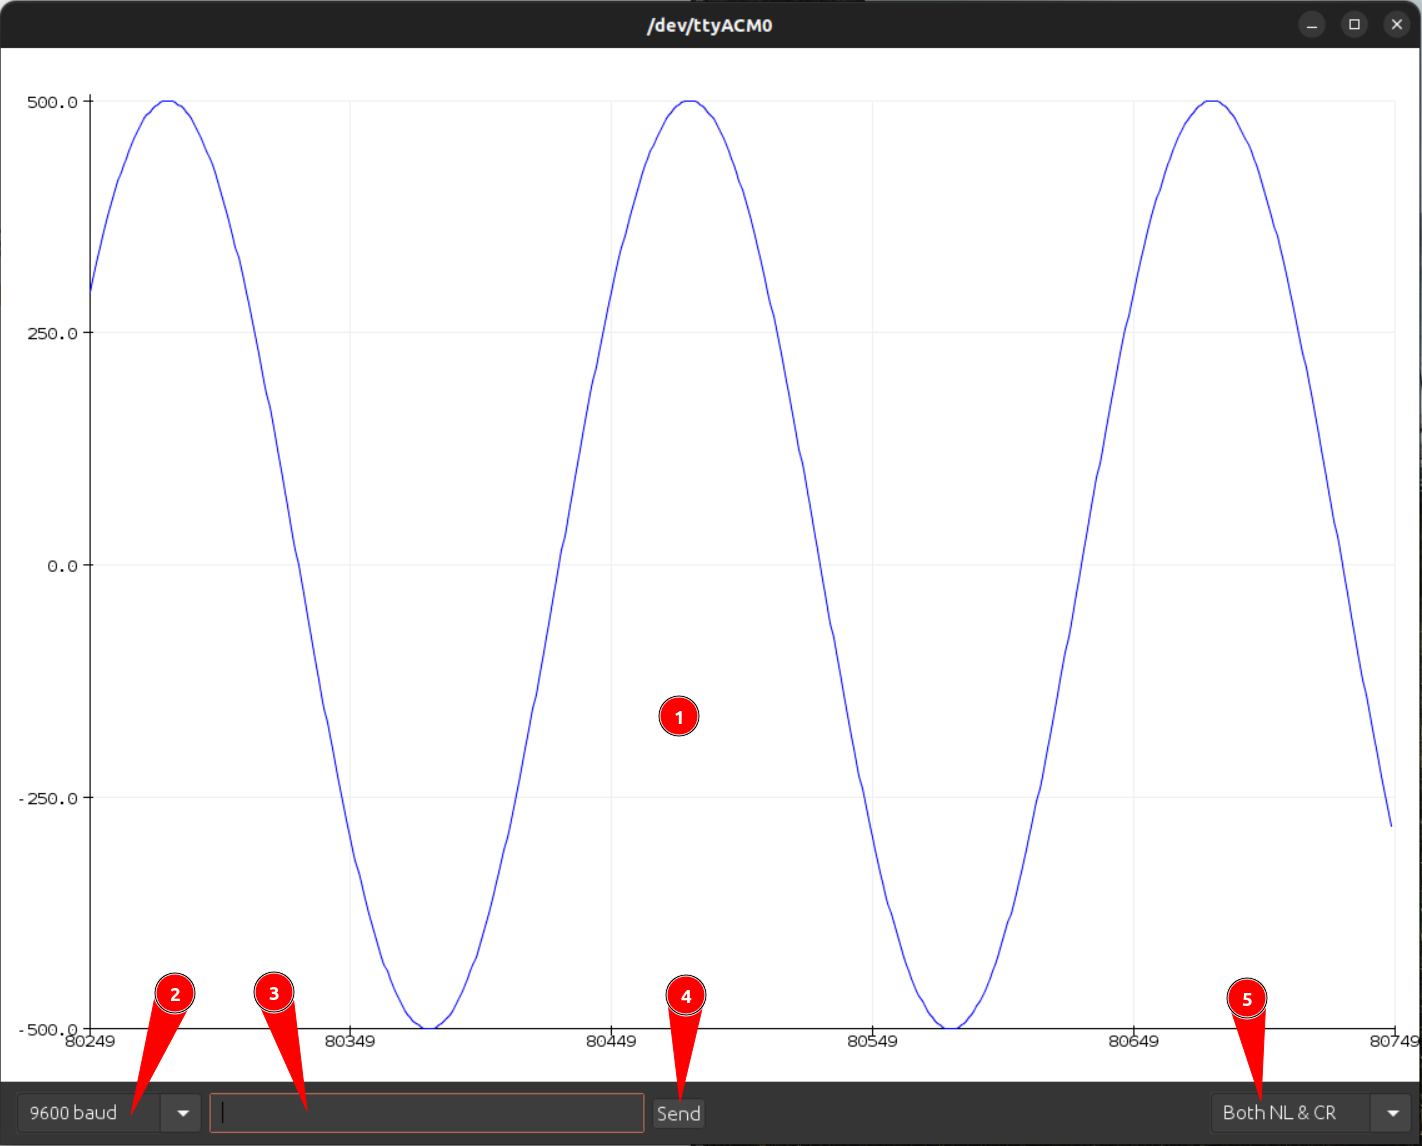
\includegraphics[width=10cm]{arduino-ide-serial-plotter}
  \caption{Плоттер по последовательному соединению (``Serial Plotter'') в
    Arduino IDE 1.8.19.}
  \label{fig:arduino-ide-serial-plotter}
\end{figure}

Цифрами на рисунке указаны:

\begin{enumerate}
\item Область отображения графика, динамически генерируемого на основе данных,
  приходящих с Arduino.
\item Настройка скорость передачи данных в бодах (битах в секунду).
  По-умолчанию выставлена в 9600 бод.  Если значение данной настройки не
  соответствует тому, который был указан в программе, работающей на Arduino
  (через \texttt{Serial.begin}), то тогда плоттер не сможет корректно отобразить
  данные.
\item Строка ввода данных для передачи их с компьютера на Arduino.
\item Кнопка ``Отправить'' (англ. ``Send''), по нажатию на которую данные,
  введённые в строку слева, будут отправлены на Arduino.
\item Настрока перевода строк, используемых при коммуникации с Arduino.  Здесь
  можно выбрать один из вариантов: ``No line ending'' (Без перевода строк),
  ``Newline'' (Перевод строки), ``Carriage return'' (Символ ``возврат каретки'')
  и ``Both NL \& CR'' (режим, в котором в роли конца строки используются сразу
  два символа -- перевод строки и возврат каретки.)  Данная опция влияет на то,
  какую последовательность символов монитор порта считает за конец строки
  данных.
\end{enumerate}

\newpage

Кстати говоря, синусоидальный график, показаный на
рис. \ref{fig:arduino-ide-serial-plotter}, был получен следующим кодом:

\begin{listing}[ht]
  \begin{minted}{cpp}
    void setup() {
      Serial.begin(9600);
    }

    int t = 0;
    void loop() {
      const double AMPLITUDE = 500;
      double y = AMPLITUDE * sin(2.0 * PI / 200 * t);
      Serial.println(y);
      t++;
      delay(1);
    }
  \end{minted}
  \label{listing:serial-port-sine-wave-example}
  \caption{Пример программы для Arduino, генерирующий синус в плоттере на
    компьютере.}
\end{listing}

\subsection{Передача данных с компьютера}

Передавать данные с Arduino на компьютер мы уже научились. Теперь посмотрим на
передачу данных в обратном направлении.  Для того чтобы передать данные с
компьютера на Arduino также необходимо выполнить настройку последовательного
порта; кроме этого, нам потребуется задействовать несколько новых функций.

\subsubsection{Чтение отдельных байт}

Функция \texttt{Serial.read} читает байт данных из поступивших на Arduino.  То
есть возвращает вам некое целое число, с которым вы вольны делать что вашей душе
угодно. Каждый вызов этого метода будет возвращать вам следующий байт данных из
тех что поступили на Arduino.  Если возвращать нечего, то есть вы считали все что
было, данная функция вернет значение -1.

\note{ Если передаются именно байты, возникает проблема: -1 это 0xFF в
  шестнадцатиричной системе, или 255 в десятичной. Такой же байт, как и все
  остальные, из-за чего невозможно. поэтому нужно сперва вызывать функцию
  \texttt{available}. }

Допустим мы отправили 1 байт данных на Arduino и использовали нижеприведенный
участок кода:

\begin{minted}{cpp}
  int incoming_byte;
  void loop() {
    if (Serial.available() > 0) {
      incoming_byte = Serial.read();
    }
  }
\end{minted}

После того, как вы считаете байт данных, он будет перемещен в вашу переменную
\texttt{incoming\_byte} а функция \texttt{Serial.available} снова будет
возвращать 0, пока не поступят новые данные.

То есть, когда вы считываете байт, показания счетчика принятых байт уменьшается
и \texttt{Serial.available} будет показывать на 1 байт меньше.

Помните, что функция \texttt{Serial.read} возвращает только 1 байт данных, если
например вы передали 4 символа каждый по 1 байту, вам потребуется 4 раза вызвать
данную функцию чтобы прочитать эти символы и самостоятельно позаботится о том
чтобы разместить их в массив символов либо воспользоваться функцией
\texttt{Serial.readBytes}.

\subsubsection{Чтение чисел}

Функция \texttt{Serial.parseInt} просматривает данные, поступившие на Arduino, и
ищет среди них набор кодов (чисел) от 48 до 57, которые соответствуют символам
чисел от 0 до 9 и преобразует все это в правильное целочисленное значение. Таким
образом если вы с монитора порта передадите ``число'' (на самом деле, строку)
``72'', данный метод увидит 2 последовательных байта 55 и 51, корректно
преобразует его в число 72 и вернет его как правильное целочисленное значение.
Давайте напишем маленькую эхо-программу, которая покажет принцип работы данной
функции и позволит вам узнать, какому символу соответствует то или иное число.

\begin{minted}{cpp}
  int incoming_int = 0;

  void setup()
  {
    Serial.begin(9600);
    Serial.setTimeout(2000);
  }

  void loop()
  {
    if (Serial.available() > 0)
    {
      incoming_int = Serial.parseInt();
      Serial.write(incoming_int);
    }
  }
\end{minted}

Мы специально поменяли с помощью функции \texttt{Serial.setTimeout} время
ожидания с 1000мс (умолчальное значение) на 2000мс, чтобы нагляднее показать
некоторые аспекты работы последовательного порта.

Примерный алгоритм работы данной программы следующий:
\begin{itemize}
  \item Если в мониторе порта вы введете строку
``72'', то монитор порта отправит её на Arduino как два байта данных в виде
чисел 55 и 51.
\item Функция \texttt{Serial.parseInt} ждёт 2000 миллисекунд.
\item После этого функция \texttt{Serial.parseInt} ``увидит'' эти два значения и
  преобразует их в одно целочисленное значение 72.
\item Произойдёт присвоение значения переменной \texttt{incoming\_int}.
\item С помощью метода \texttt{Serial.write} программа передаёт значение
  переменной \texttt{incoming\_int} (число 72 в данном примере) обратно на
  комьпьютер.
\item На компьютере монитор порта корректно преобразует число 72 в
  соответствующий символ и покажет нам символ ``H'' который соответствует коду
  72.
\end{itemize}

\subsection{Задачи}

\begin{enumerate}
\item Попробуйте модифицировать исходный код из примера
  \ref{listing:serial-port-sine-wave-example}, генерирующей синус (как на
  рис. \ref{fig:arduino-ide-serial-plotter}) таким образом, чтобы амплитуда
  графика была больше.
\item Модифицируйте также код, чтобы период синусоиды был меньше (иными словами,
  чтобы частота была выше.)
\item Сделайте вывод двух синусоид одновременно таким образом, чтобы они
  находились в противофазе.
\end{enumerate}

\end{document}
